\section{Four stones in a row}\label{sec:geometry}

The certificate establishes the empty-board theorem without assuming
that nearby Breaker cells stay sparse. A separate local statement
explains some of the geometry behind its threats. The perpendicular
attack below is related to the four-in-a-row tactics of Halupczok
and Schlage-Puchta \cite[Section~3, pp.~13--15]{HSP2007}; their planar
row extensions also appear in Sections~4.4--4.6 of that paper.
We give a complete proof for the precise finite-neighborhood
hypothesis used here.

\begin{proposition}\label{prop:four-row}
Suppose it is Maker's turn at an arbitrary finite position, Maker
owns the four cells
\[
 \{(0,0),(1,0),(2,0),(3,0)\},
\]
and Breaker owns at most three cells in
\[
 Q=([-3,6]\times[-4,4])\cap\Z^2.
\]
Then Maker has already won or can force a win. Additional Maker
cells and arbitrary Breaker cells outside $Q$ are allowed.
\end{proposition}

Call a set \emph{clean} if it contains no Breaker cell.
Throughout this section, an instruction to claim an already-owned
Maker cell means to claim any free cell instead, unless a target
has already been completed. Such a replacement is a real move and
allows exactly one new Breaker reply. Extra Maker cells therefore
cause no difficulty in any of the arguments below.

When a move is said to force Breaker to a cell $q$, the precise
meaning is that $q$ completes an allowed target on Maker's next
move. If $q$ is already Maker's, the target is already complete.
Otherwise $q$ is free, and Breaker must claim it or allow that
immediate completion. Every forced continuation is considered only
when Maker has not already won or obtained this next-move win.

\subsection{A five-cell fork}

Suppose Maker owns the horizontal five
$\{(r,0),\ldots,(r+4,0)\}$. For an endpoint $e\in\{r,r+4\}$
and a sign $\varepsilon\in\{-1,1\}$, put
\begin{equation}\label{eq:horizontal-triple}
 H(e,\varepsilon)=
 \{(e-1,\varepsilon),(e,\varepsilon),(e+1,\varepsilon)\}.
\end{equation}
If this triple is clean at Maker's turn, claiming its middle cell
$(e,\varepsilon)$ creates two one-cell completions, at its other
two cells. The two targets use respectively the first and last
four-cell subrows of the five; they are reflected or translated
copies of $S$. Breaker can occupy at most one completion, so
Maker wins on the next move unless it has already won.
This is the horizontal version of Figure~\ref{fig:fork}.

The four triples in \eqref{eq:horizontal-triple} are pairwise
disjoint. Consequently, if Maker has just created the five and
at least two of these triples are clean \emph{before} Breaker's
response, at least one remains clean afterwards, and the fork
wins. The same assertion holds after interchanging the coordinates.
For a vertical five we use the notation
\[
 V(c,d)=\{(c,d-1),(c,d),(c,d+1)\},
\]
where $c\in\{-1,1\}$ and $d$ is an endpoint height.

\subsection{The perpendicular endpoint attack}

We first establish a local tactic at the right endpoint of a row.
Assume Maker owns the four cells
\[
 (-3,0),\quad(-2,0),\quad(-1,0),\quad(0,0),
\]
and the set
\begin{equation}\label{eq:endpoint-zone}
 Z=\{(x,y):x\in\{-1,0,1\},\ 1\le |y|\le4\}
\end{equation}
is clean. Other ownership is arbitrary.
Maker claims $(0,1)$, forcing $(1,1)$, and then $(0,-1)$,
forcing $(1,-1)$. Indeed, the original horizontal body with the
respective pair of cells above or below its endpoint is an allowed
Snaky. If Breaker declines either forced reply, Maker completes
that copy on its next turn.

After those two replies, Maker claims $(0,2)$. Denote the new
Breaker reply by $b$, and set
\[
E=\{(0,-2)\}\cup V(-1,-2)\cup V(-1,2).
\]
Figure~\ref{fig:endpoint-branches} separates the two possible
continuations after this reply.
If $b\notin E$, Maker claims $(0,-2)$. It now owns the vertical
five from height $-2$ to height $2$, and both $V(-1,-2)$ and
$V(-1,2)$ are clean before the ensuing Breaker reply. They are
disjoint, and neither of the two earlier forced Breaker cells is
in either triple. The five-cell fork therefore wins.

If $b\in E$, Maker instead claims $(0,3)$, creating the vertical
five from height $-1$ to height $3$. The triple $V(1,3)$ is clean.
The triple $V(-1,3)$ is also clean unless
\[
 b=(-1,2)\quad\hbox{or}\quad b=(-1,3).
\]
If both are clean, the same two-triple argument wins.
In either exceptional case there is instead an immediate
completion at $q=(-1,-1)$, because Maker already owns the other
five cells of
\begin{equation}\label{eq:perpendicular-copy}
 \{(0,3),(0,2),(0,1),(0,0),(-1,0),(-1,-1)\}
 =\{(-y,3-x):(x,y)\in S\}.
\end{equation}
The cell $q$ lies in the initially clean zone, and differs from
$b$ and from the two earlier forced replies. It is thus free
unless Maker already owns it, in which case the target is complete.
It also lies outside $V(1,3)=\{(1,2),(1,3),(1,4)\}$.
Breaker must either claim $q$, leaving that clean triple for the
five-cell fork, or leave $q$ as an immediate winning move.
This completes the endpoint tactic.

\begin{figure}[tb]
\centering
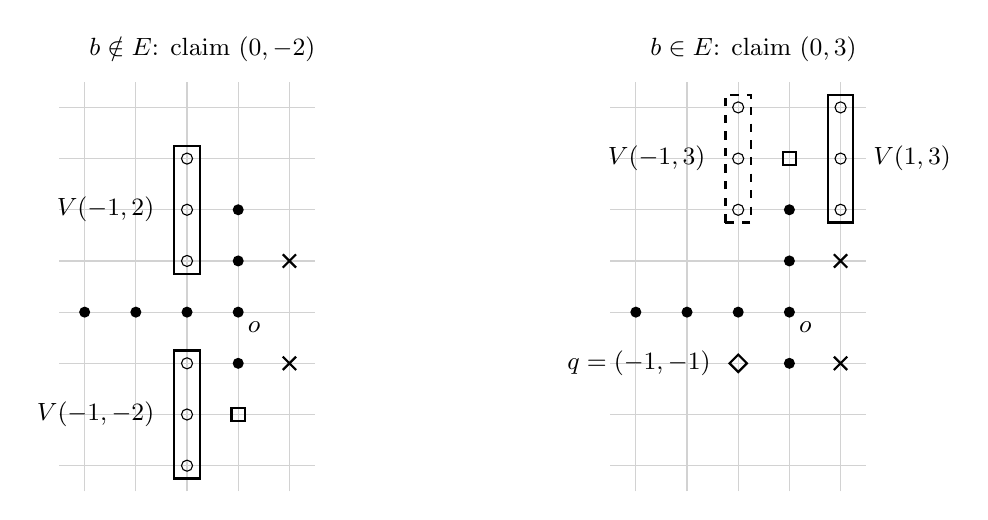
\begin{tikzpicture}[x=6.5mm,y=6.5mm,font=\small]
\foreach \shift in {0,7}{
 \begin{scope}[xshift=\shift cm]
 \draw[gray!35,step=1] (-3.5,-3.5) grid (1.5,4.5);
 \foreach \x/\y in {-3/0,-2/0,-1/0,0/0,0/-1,0/1,0/2}
  {\fill (\x,\y) circle (2pt);}
 \foreach \y in {-1,1}
  {\draw[thick] (.87,\y-.13)--(1.13,\y+.13)
                (.87,\y+.13)--(1.13,\y-.13);}
 \node[below right] at (0,0) {$o$};
 \end{scope}
}
\begin{scope}
\node[above] at (-.7,4.7) {$b\notin E$: claim $(0,-2)$};
\draw[thick] (-1.25,-3.25) rectangle (-.75,-.75);
\draw[thick] (-1.25,.75) rectangle (-.75,3.25);
\foreach \y in {-3,-2,-1,1,2,3}
 {\draw (-1,\y) circle (2pt);}
\draw[thick] (-.13,-2.13) rectangle (.13,-1.87);
\node[left] at (-1.45,-2) {$V(-1,-2)$};
\node[left] at (-1.45,2) {$V(-1,2)$};
\end{scope}
\begin{scope}[xshift=7cm]
\node[above] at (-.7,4.7) {$b\in E$: claim $(0,3)$};
\draw[thick,dashed] (-1.25,1.75) rectangle (-.75,4.25);
\draw[thick] (.75,1.75) rectangle (1.25,4.25);
\foreach \x in {-1,1}
 \foreach \y in {2,3,4}{\draw (\x,\y) circle (2pt);}
\draw[thick] (-.13,2.87) rectangle (.13,3.13);
\draw[thick] (-1,-.83)--(-.83,-1)--(-1,-1.17)--(-1.17,-1)--cycle;
\node[left] at (-1.45,3) {$V(-1,3)$};
\node[right] at (1.45,3) {$V(1,3)$};
\node[left] at (-1.35,-1) {$q=(-1,-1)$};
\end{scope}
\end{tikzpicture}
\caption{Alternative endpoint continuations after the reply $b$,
which is not drawn; here $o=(0,0)$. Dots show guaranteed Maker cells,
crosses the two earlier forced Breaker cells, and each square the
prescribed next claim.
Solid outlines enclose clean triples, whose cells may already be
Maker-owned. On the left, their union with the square is $E$.
On the right, the dashed triple is clean except when
$b=(-1,2)$ or $b=(-1,3)$; in those cases, claiming $(0,3)$
leaves the diamond $q$ as an immediate completion while $V(1,3)$ stays
clean. The panels are conditional alternatives, not consecutive moves.}
\label{fig:endpoint-branches}
\end{figure}

Every prescribed target or threat cell in this tactic lies in
$\{-3,-2,-1,0\}\times\{0\}$ or in $Z$.
Fresh replacement moves may be elsewhere on the board.
In particular, arbitrary Breaker moves outside the stated zone
are included in the preceding cases and cannot defeat the tactic.

\subsection{Proof of the four-in-a-row result}

\begin{proof}[Proof of Proposition~\ref{prop:four-row}]
Assume no target is already complete, and consider the two
extensions $(-1,0)$ and $(4,0)$ of the given row.

If both extensions belong to Breaker, there is at most one further
old Breaker cell in $Q$. The endpoint tactic has two possible
placements: at the left endpoint use $(x,y)\mapsto(-x,y)$, and
at the right endpoint use $(x,y)\mapsto(x+3,y)$.
Their off-row zones are respectively
\[
 \{-1,0,1\}\times\{-4,-3,-2,-1,1,2,3,4\}
 \quad\hbox{and}\quad
 \{2,3,4\}\times\{-4,-3,-2,-1,1,2,3,4\}.
\]
They are disjoint subsets of $Q$, and neither contains the two
row blockers. At least one zone is clean. The corresponding
endpoint tactic proves the result.

If exactly one extension belongs to Breaker, claim the other.
This produces a five in a row. The four endpoint triples are
pairwise disjoint and all lie in $Q$. The old row blocker meets
none of them, and at most two further old Breaker cells can meet
them. Thus at least two triples are clean before the new Breaker
response, and the five-cell fork wins.

It remains to consider the case that neither extension belongs
to Breaker. If one extension produces a five with at least two
clean endpoint triples, use it and finish as above. Suppose that
both choices fail this test. For extension to the left, the four
triples are $H(-1,\pm1),H(3,\pm1)$; for extension to the right,
they are $H(0,\pm1),H(4,\pm1)$.
Failure of either test requires at least three of its disjoint
triples to contain an old Breaker cell. Since at most three old
Breaker cells lie in $Q$, there are exactly three, and each must
meet a triple for both tests. A cell with this property lies on
level $-1$ or $1$ and has its first coordinate in $\{-1,0\}$
or in $\{3,4\}$. Moreover, their three combinations of
\emph{left or right cluster} and \emph{lower or upper level}
are distinct; otherwise fewer than three disjoint triples would
be met in one of the tests.

The reflections $(x,y)\mapsto(3-x,y)$ and
$(x,y)\mapsto(x,-y)$ preserve both the original four-cell row
and $Q$. They allow us to take the missing cluster-level
combination to be the lower right one. The three old Breaker
cells then have the form
\begin{equation}\label{eq:three-blockers}
 (l_-,-1),\quad(l_+,1),\quad(r,1),
 \qquad l_-,l_+\in\{-1,0\},\quad r\in\{3,4\}.
\end{equation}
No other old Breaker cell lies in $Q$.
Let $a$ count the true statements $l_-=0$, $l_+=0$, and $r=4$.

Suppose first that $a\ge2$. Claim $(-1,0)$.
The resulting five from $-1$ to $3$ has the clean triple
$H(3,-1)$. Unless Breaker meets it on its next move, Maker
uses that fork. Hence we may assume Breaker's new cell belongs
to $H(3,-1)=\{(2,-1),(3,-1),(4,-1)\}$.
Claim $(-2,0)$, which is free or already Maker's: neither an
old blocker nor that new cell can occupy it.
For the five from $-2$ to $2$, each of the following is a clean
endpoint triple when its indicated condition holds:
\[
\begin{array}{c|c}
\text{triple}&\text{condition}\\ \hline
H(-2,-1)&l_-=0\\
H(-2,1)&l_+=0\\
H(2,1)&r=4.
\end{array}
\]
They are pairwise disjoint and are all missed by the last
Breaker move. There are at least $a\ge2$ such triples before
the next response. The five-cell fork wins.

If $a\le1$, claim $(4,0)$ instead. Its clean lower-right triple
$H(4,-1)$ forces the next Breaker cell into
$\{(3,-1),(4,-1),(5,-1)\}$, or gives an immediate fork win.
Claim $(5,0)$, again free or already Maker's.
For the five from $1$ to $5$, the clean disjoint triples are
\[
\begin{array}{c|c}
\text{triple}&\text{condition}\\ \hline
H(1,-1)&l_-=-1\\
H(1,1)&l_+=-1\\
H(5,1)&r=3.
\end{array}
\]
At least $3-a\ge2$ conditions hold, and the most recent Breaker
cell meets none of these triples. The fork again wins.
All extension cells and triples in both cases lie in $Q$.
This exhausts the possibilities and proves the proposition.
\end{proof}

Proposition~\ref{prop:four-row} is a sufficient condition at an
arbitrary Maker turn. Its proof does not assume that the four
stones were obtained consecutively, and the $21$-move theorem
does not assume that its three-blocker hypothesis occurs during
play. The full certificate supplies the empty-board strategy.
